\section{Initial and boundary conditions}\label{pocatecni a okrajove podminky}

The choice of initial and boundary conditions is an integral part of the lattice Boltzmann method to ensure consistency the mesoscopic description. Therefore, the chosen initial and boundary conditions are described in more detail in this section.

\subsection{Initial condition}\label{pocatecni podminka}
Let us now consider the domain defined by relations \eqref{eq:domain}. In this work, the equilibrium distribution function \( f^{\mathrm{eq}} \) is used to set the initial condition. The equilibrium distribution function is given by
\begin{equation}\label{eq:feq}
	f^{\mathrm{eq}}_{k} = \rho w_{k} \, \left(1 + \frac{\vec{\xi_{k}} \cdot \vec{u}}{c^{2}_{s}} + \frac{(\vec{\xi_{k}} \cdot \vec{u})^2}{2c^{4}_{s}} - \frac{\vec{u} \cdot \vec{u}}{2c^{2}_{s}} \right)\, , \hspace{2mm} k \in \{1,\dots,27\},
\end{equation}
where \( w_{k} \) are the weights specific to the chosen velocity model. For the D3Q27 model, these weights are defined as \cite{Kruger}
\begin{equation}
	w_k= \begin{cases}\frac{8}{27}, & k=1, \\ \frac{2}{27}, & k = 2,3, \ldots, 7, \\ \frac{1}{54}, & k = 8,9, \ldots, 19, \\ \frac{1}{216}, & k = 20,21, \ldots, 27.\end{cases}
\end{equation}
The initial density \( \rho \) and the velocity \( \vec{u} \), are denoted as \( \rho _{\mathrm{ini}} \) and \( \vec{u} _{\mathrm{ini}} \), respectively. At each lattice node \( \vec{x} \in \hat{\Omega} \) at time \( t=0 \), the distribution functions are initialized as
\begin{equation}\label{eq:initial condition}
	f^{}_{k} (\vec{x}, 0) = f^{\mathrm{eq}}_{k} (\rho _{\mathrm{ini}} (\vec{x}), \vec{u} _{\mathrm{ini}} (\vec{x})), \hspace{3mm} k \in \{1, \dots 27\}.
\end{equation}

This approach assumes that the non-equilibrium component of the distribution functions, defined as \( f^{\mathrm{neq}}_{k} = f_{k} - f^{\mathrm{eq}}_{k} \), can be neglected, and the distribution functions can be approximated by their equilibrium part. A significant advantage of this choice of initial condition approximation is its easy implementation. While more advanced initialization methods exist  \cite{PE}, the equilibrium-based approach is used in this work.

\subsection{Boundary conditions}


\subsubsection*{Bounce-back boundary condition}\label{bounce-back}
The first boundary condition discussed is the bounce-back boundary condition, specifically its \textit{fullway} variant \cite{Kruger}. The bounce-back boundary condition is typically used for modeling the interface between a fluid and a solid. Its advantage is that it satisfies the no-slip condition at the fluid-solid interface while remaining straightforward to implement. The principle of the bounce-back boundary condition is that at the interface, the distribution functions corresponding to particles with microscopic velocity \( \vec{\xi_{k}} \) are reflected back into the directions from which they arrived at the node, with velocity \( \vec{\xi_{\bar{k}}} = -\vec{\xi_{k}} \).

When using this boundary condition, the fluid-solid interface is located halfway between the fluid and solid nodes. For curved boundaries that are not parallel to the grid, the bounce-back method leads to a "staircase" shape of the boundary, which can limit the accuracy of the simulation.

In this approach, particles are reflected over two time steps. During this time, the particles reach the solid nodes, where their direction is reversed and they are streamed back, as schematically shown in Figure \ref{fig:fbb}.

\begin{figure}[h]
%	\vspace{-.5cm}
	\centering

	\begin{subfigure}{0.48\textwidth}
		\centering
		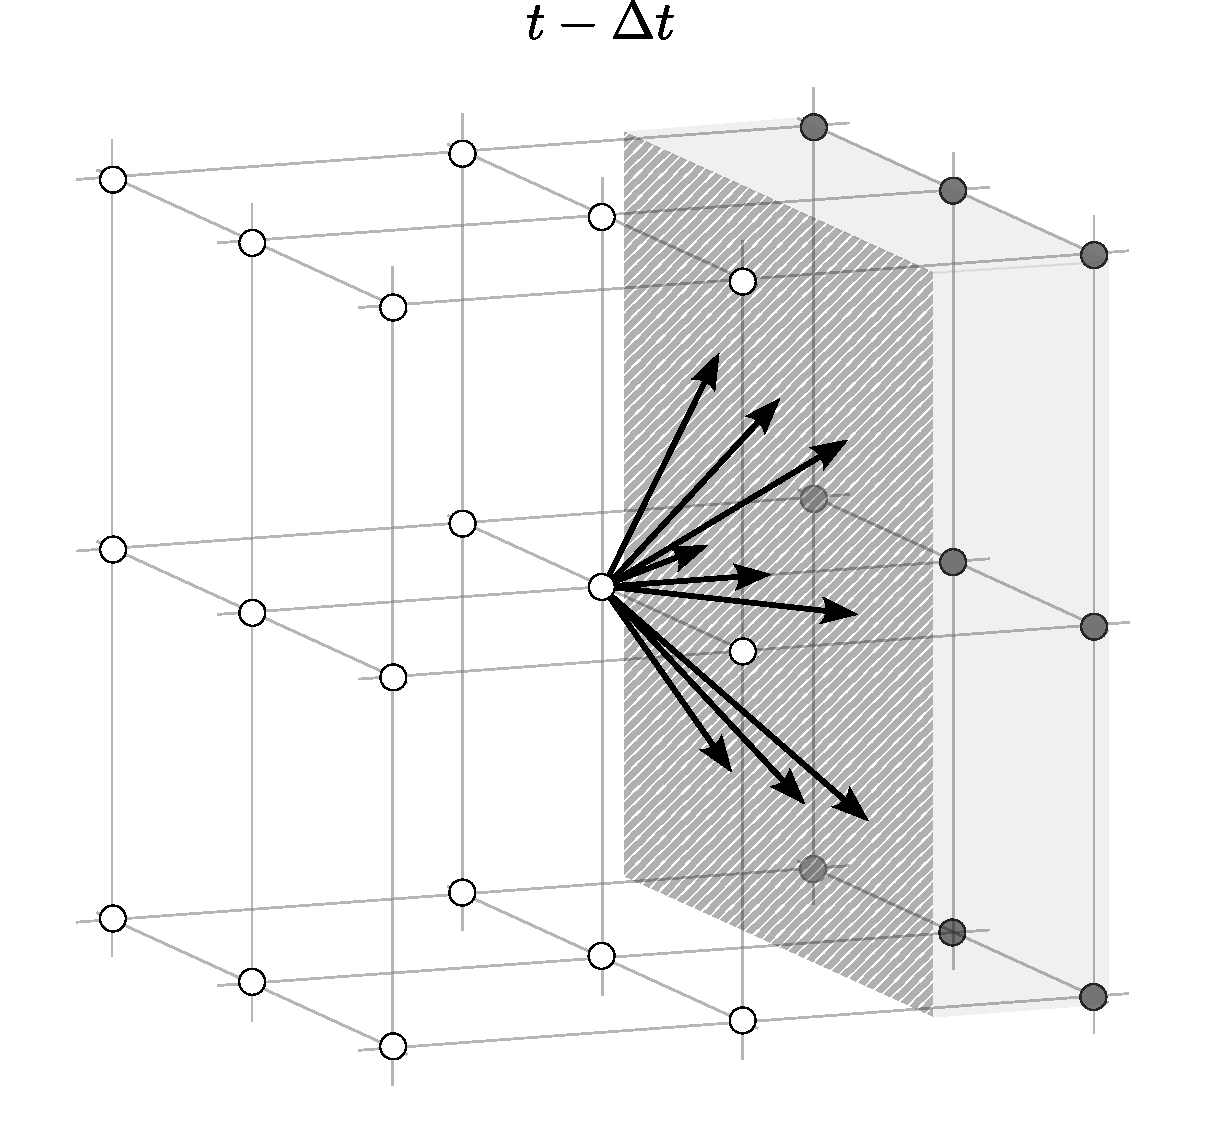
\includegraphics[width=0.9\textwidth, trim={0mm 0mm 0mm 0mm}]{figures/fwbba.pdf}
		\caption{Step before the streaming at time $t - \Delta t$.}
		\label{fig:bba}
	\end{subfigure}
	\begin{subfigure}{0.48\textwidth}
		\centering
		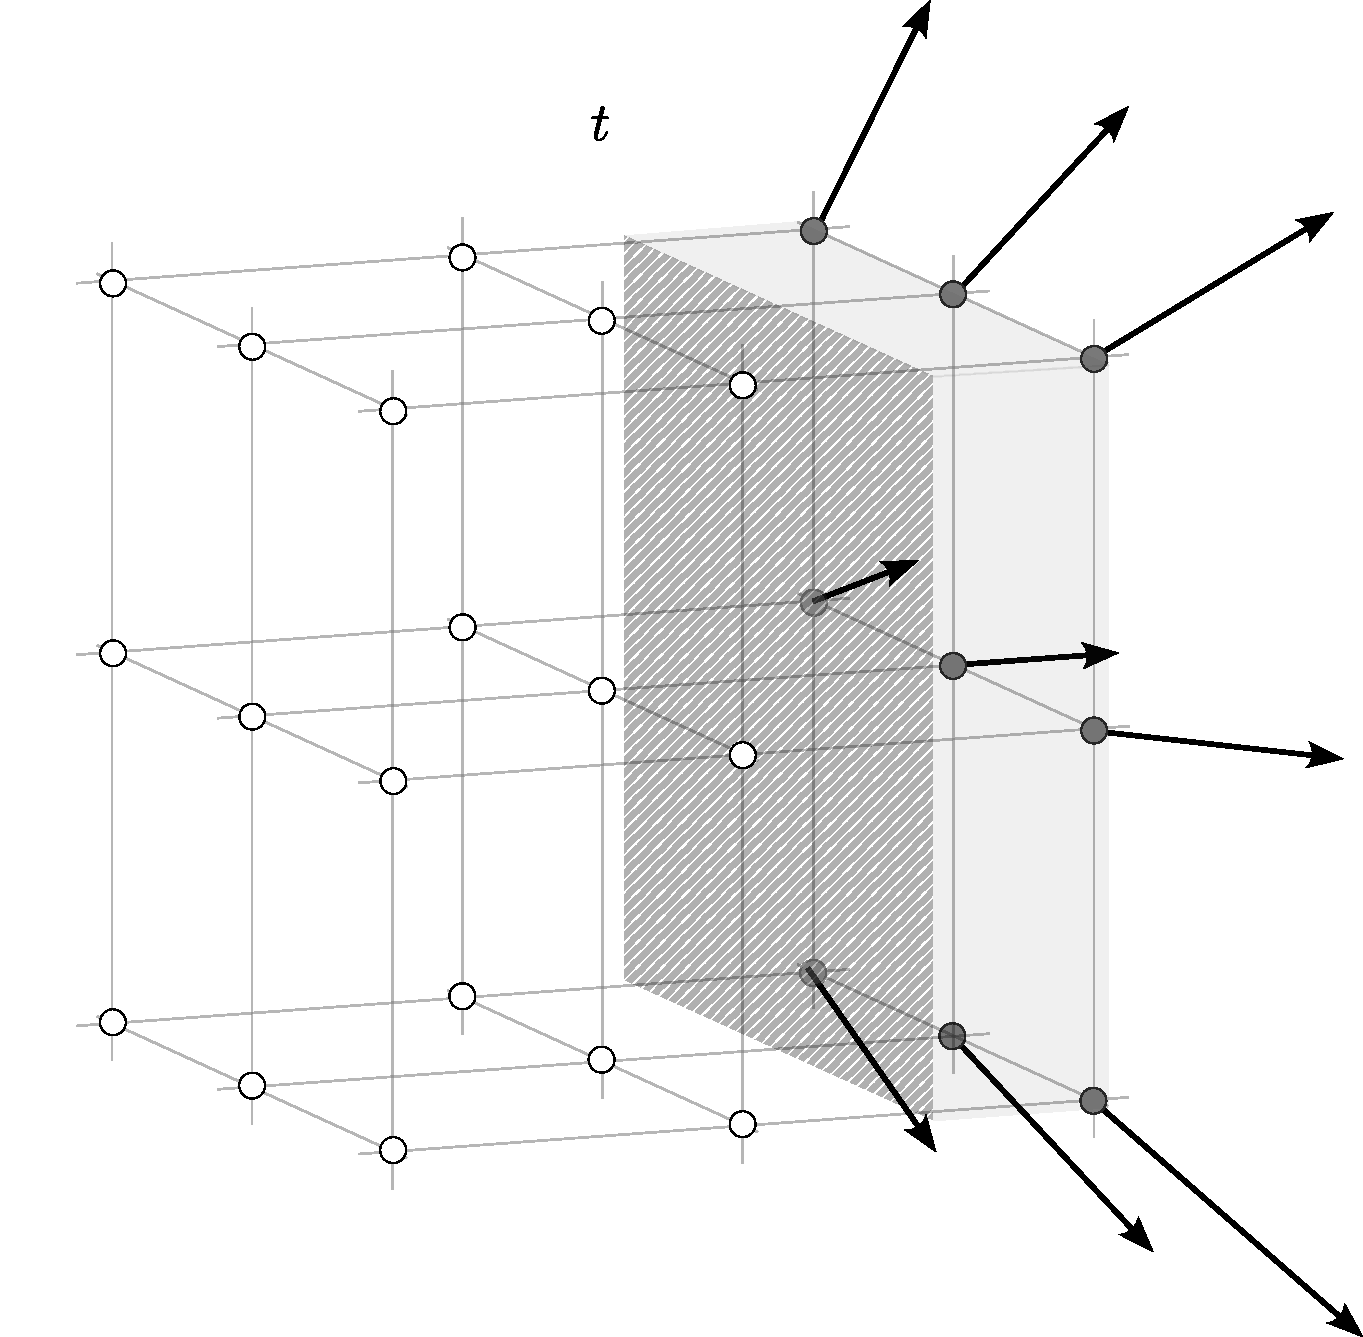
\includegraphics[width=0.9\textwidth, trim={0mm 0mm 0mm 0mm}]{figures/fwbbb.pdf}
		\caption{Step after streaming at time $t$.}
		\label{fig:bbb}
	\end{subfigure}
	\par\bigskip
	\par\bigskip
	\begin{subfigure}{0.48\textwidth}
		\centering
		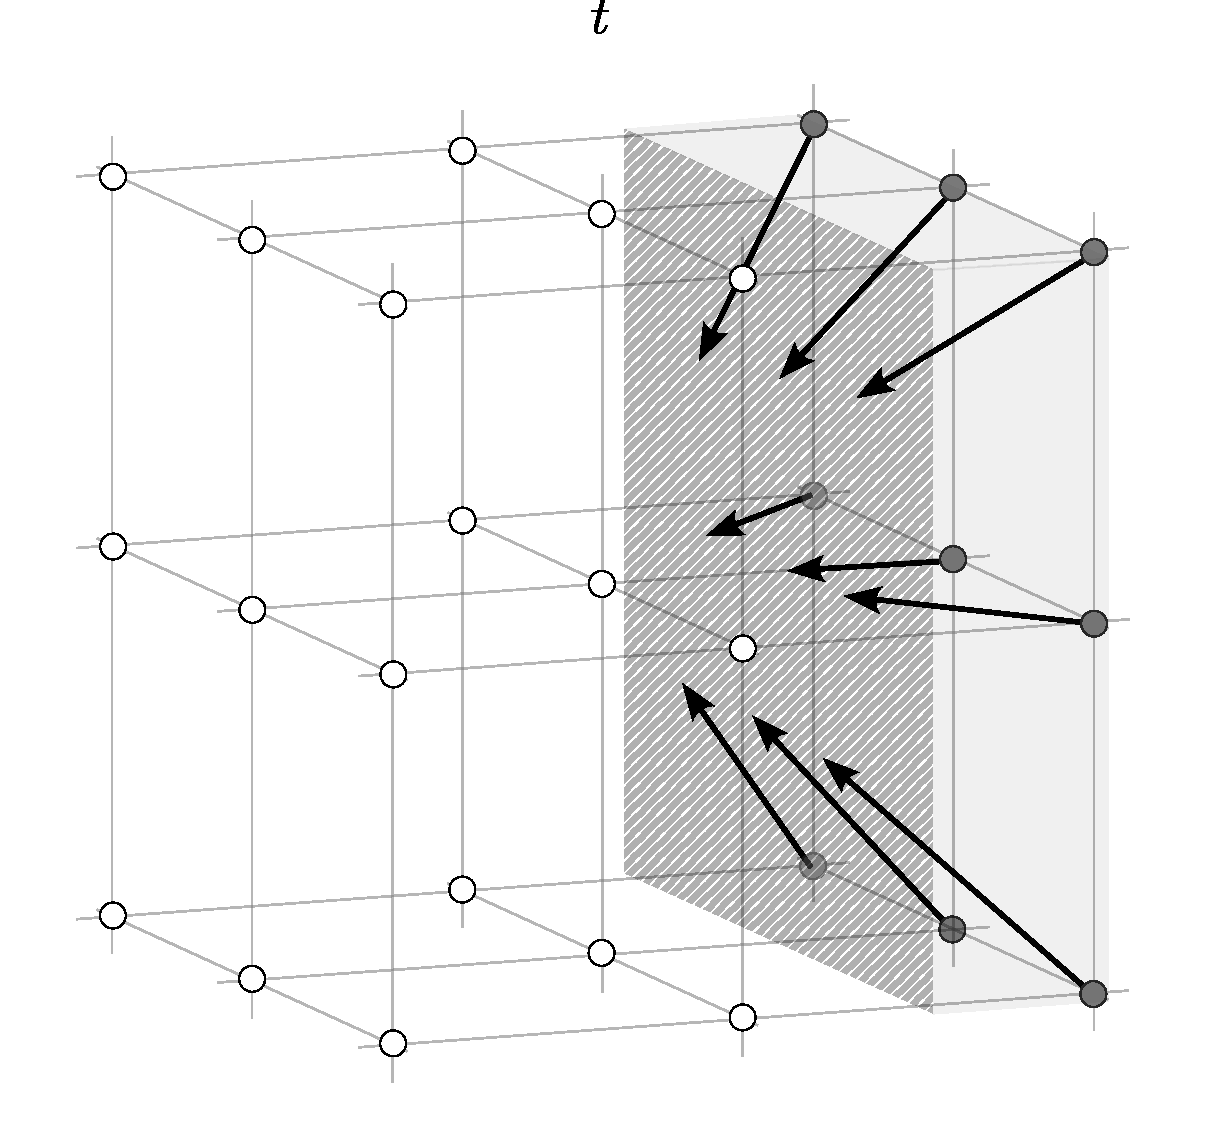
\includegraphics[width=0.9\textwidth, trim={0mm 0mm 0mm 0mm}]{figures/fwbbc.pdf}
		\caption{The distribution functions are reversed.}
		\label{fig:bbc}
	\end{subfigure}
	\begin{subfigure}{0.48\textwidth}
		\centering
		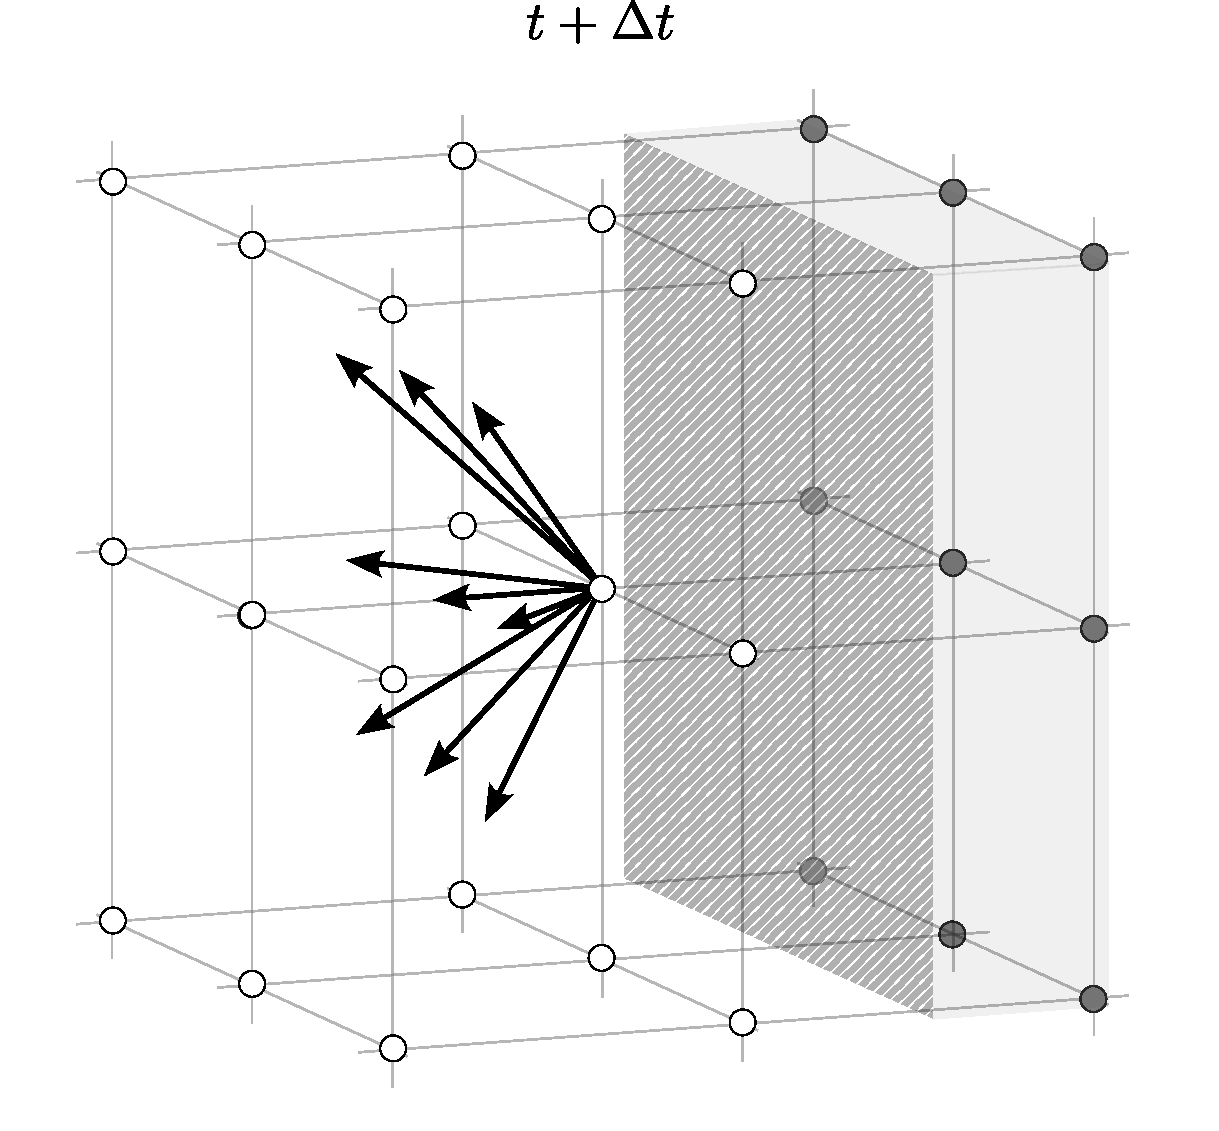
\includegraphics[width=0.9\textwidth, trim={0mm 0mm 0mm 0mm}]{figures/fwbbd.pdf}
		\caption{Step after the streaming at time $t + \Delta t$.}
		\label{fig:bbd}
	\end{subfigure}
	\vspace{5mm}
	\caption{Schematic representation of the fullway bounce-back boundary condition for the D3Q27 velocity model. White points represent fluid nodes, and gray points represent wall nodes. The wall is represented by a gray plane.}
	\label{fig:fbb}
\end{figure}

An alternative to the fullway method is the \textit{halfway} variant of the bounce-back boundary condition, which completes the reflection process within a single time step. Details can be found in \cite{Kruger}. In this work, however, we limit ourselves to the fullway variant.

%\subsubsection{Equilibrium boundary condition}\label{equilibrium bc}
%One option for approximating unknown distribution function values at the boundary nodes is to use the equilibrium distribution function, defined as \cite{PE}
%\begin{equation}
%	f_i(\vec{x}, t)=f_{i}^{\text{(eq)}}(\rho(\vec{x}, t), \vec{u}(\vec{x}, t)), \hspace{2mm}  \forall k \in \{1,\dots,27\}, \forall t \in \hat{\mathcal{I}}.
%\end{equation}
%The advantage of this approximation is its simple implementation, while the disadvantage is the neglect of the non-equilibrium part of the distribution function \cite{PE}.

%\subsubsection{Symmetric boundary condition}\label{symmetric bc}
%The symmetric boundary condition assumes that the domain is symmetric relative to a given mirror plane. This boundary condition can be understood as a bounce-back-like method. The distribution functions leave the boundary node at time $t$, meet the symmetry surface at time $t + \frac{\Delta t}{2}$, where they are mirrored, and return to the fluid nodes at time $t + \Delta t$. The components of the mirrored velocity depend on the normal vector of the symmetry plane, the tangential components of the velocity remain unchanged. The symmetric boundary condition is illustrated in Figure~\ref{fig:symmetric bc}.
%\vspace{2mm}
%\begin{figure}[H]
%	\centering
%	\begin{subfigure}{0.47\textwidth}
%		\centering
%		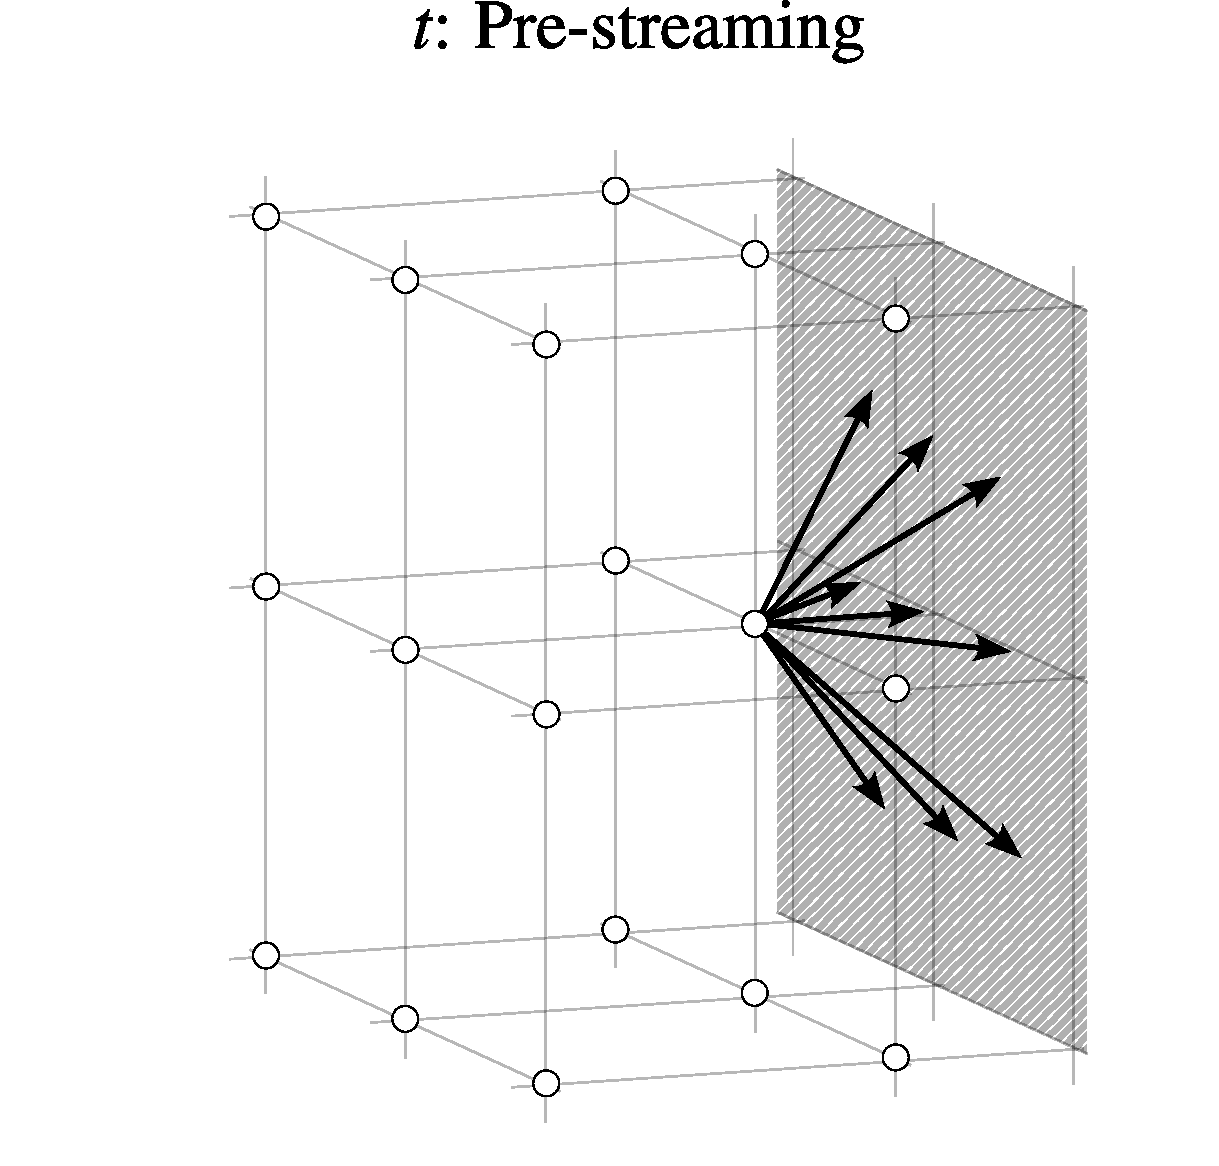
\includegraphics[width=0.99\textwidth, trim={0mm 0mm 0mm 0mm}]{figures/symmetric-a.pdf}
%		\caption{The distribution functions leave the boundary node at time $t$.}
%		\label{fig:sym a}
%	\end{subfigure}\hfill% 
%	\begin{subfigure}{0.47\textwidth}
%			\centering
%			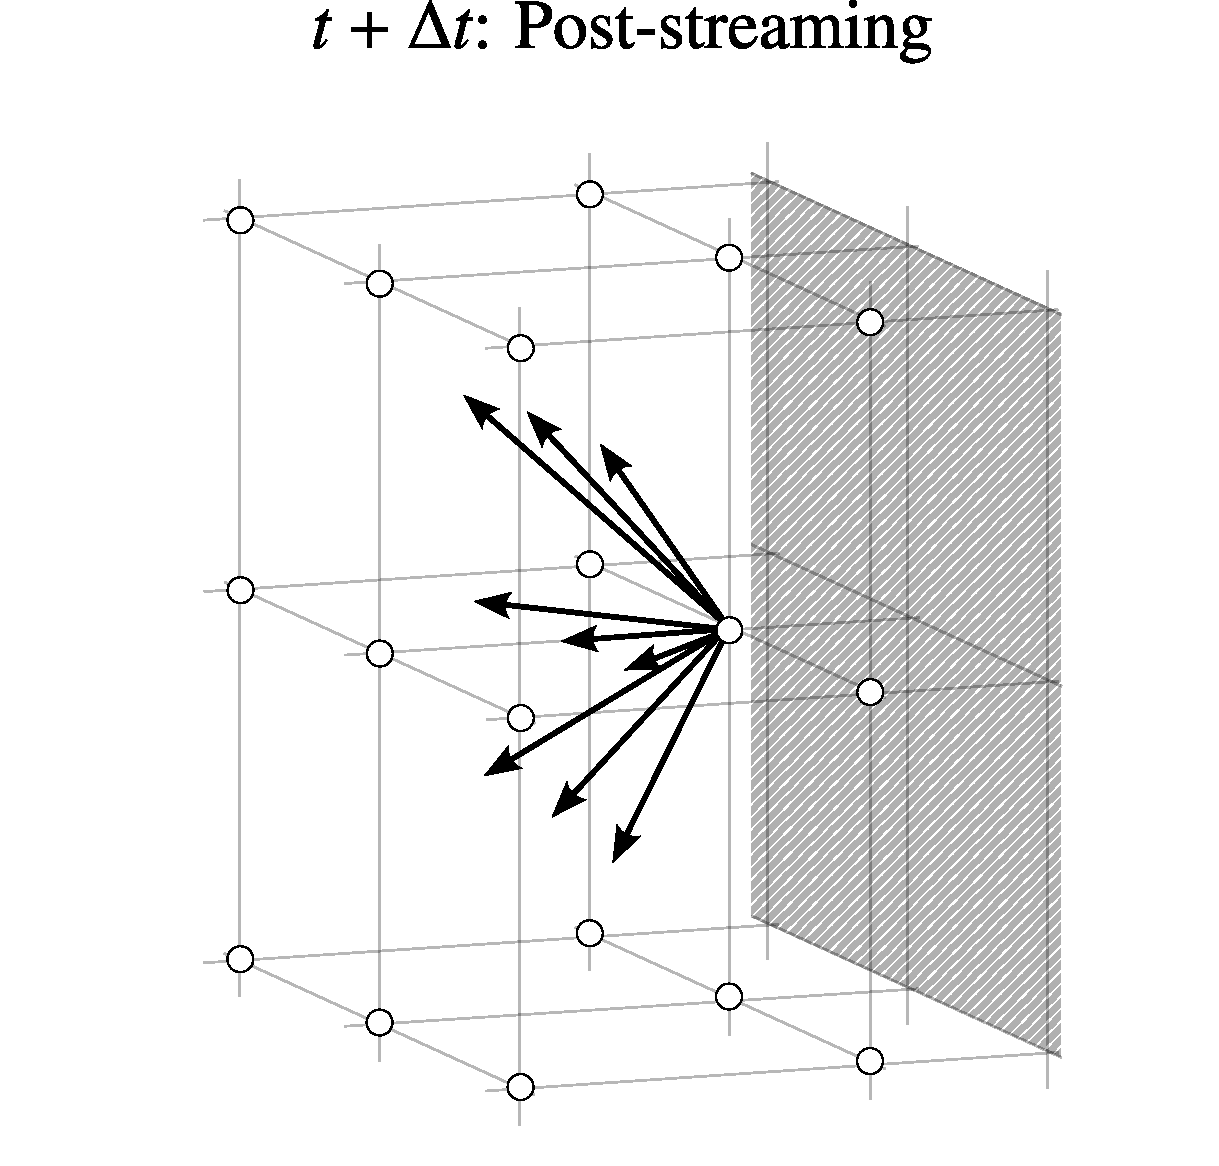
\includegraphics[width=0.99\textwidth, trim={0mm 0mm 0mm 0mm}]{figures/symmetric-b.pdf}
%			\caption{The mirrored distribution functions return to fluid nodes at time $t + \Delta t$.}
%			\label{fig:sym b}
%	\end{subfigure}
%	\vspace{2mm}
%	\caption{Illustration of the symmetric boundary condition for the symmetry plane with the normal vector \( (-1, 0, 0) \) using the D3Q27 velocity model. White points represent fluid nodes, and gray plane resents the symmetry plane.}
%	\label{fig:symmetric bc}
%
%\end{figure}

\subsubsection*{Free outflow boundary condition}\label{symmetric bc}
When using the free outflow boundary condition at the outlets, each distribution function for directions pointing out of the domain is set equal to the value it had at the adjacent node inside the computational domain in the previous timestep. While this boundary condition is numerically stable, its usage can cause unphysical behavior of pressure and velocity field near the outflow boundary. Details on the free outflow boundary condition can be found in \cite{PE}.